%(BEGIN_QUESTION)
% Copyright 2009, Tony R. Kuphaldt, released under the Creative Commons Attribution License (v 1.0)
% This means you may do almost anything with this work of mine, so long as you give me proper credit

Examine this P\&ID and answer the following questions:

$$\includegraphics[width=15.5cm]{i04197x01.eps}$$

\vskip 10pt

Identify the ``normal'' mode of operation for this system as specified by the process engineer who built it: the status of the process valve and of both solenoid valves during typical process operations.

\vskip 10pt

Identify the ``normal'' mode of operation for each solenoid valve as specified by the solenoid manufacturer: the status of each solenoid valve when it is in a condition of rest (no stimulation).

\vskip 10pt

Explain what type of electrical signal status (power applied or power removed) is required at each solenoid valve to ``trip'' the process valve from its regular operating position.  Must both solenoids change state to trip the process valve (2oo2 to trip), or is one sufficient (1oo2 to trip)?

\vskip 20pt \vbox{\hrule \hbox{\strut \vrule{} {\bf Suggestions for Socratic discussion} \vrule} \hrule}

\begin{itemize}
\item{} The usage of the word ``normal'' is very different when describing a solenoid coil's energization state versus when the same word is used to describe a spring-return valve being ``normally-open'' or ``normally-closed.''  Explain how these two meanings differ, and why this distinction -- though confusing it may be -- is important to understand.
\item{} Explain the significance of the linetypes used in this diagram.
\item{} Identify the type of process valve used in this system, from the symbol.
\item{} If you have studied mathematical probability as it applies to system reliability, calculate the probability of the process valve shutting off when it shouldn't (i.e. this trip system's {\it unsecurity}) given the following probabilities of component failure:
\itemitem{} $P$ of first solenoid valve accidently venting air pressure = 0.02
\itemitem{} $P$ of second solenoid valve accidently venting air pressure = 0.01
\itemitem{} $P$ of instrument air supply failing = 0.05
\item{} If you have studied mathematical probability as it applies to system reliability, calculate the probability of the process valve shutting off during an emergency (trip) condition (i.e. this trip system's {\it dependability}) given the following component dependability figures:
\itemitem{} $P$ of first solenoid valve dependably venting air pressure = 0.99
\itemitem{} $P$ of second solenoid valve dependably venting air pressure = 0.97
\end{itemize}

\underbar{file i04197}
%(END_QUESTION)





%(BEGIN_ANSWER)


%(END_ANSWER)





%(BEGIN_NOTES)

The design engineer made it so that air will pass to the process valve actuator during typical (good) operating conditions, holding the process valve open.

\vskip 10pt

This is a 1oo2 to trip system, because the process valve will go to its ``fail'' position if either of the two solenoid valves trip (go to their abnormal operating states).





\vskip 20pt \vbox{\hrule \hbox{\strut \vrule{} {\bf Virtual Trip-testing} \vrule} \hrule}

This question is a good candidate for a ``Virtual Trip-testing'' exercise.  Presenting the diagram to students, you pose an assignment whereby students must figure out how to test some component of this system to check that it will operate as intended to shut down the system in an abnormal (trip) condition, with some realistic limitation (e.g. power cannot be shut off to the load).  Students then propose various methods for executing the test.  Your job is to determine whether or not their proposed tests will achieve the desired result(s).

During and after the exercise, it is good to ask students follow-up questions such as:

\begin{itemize}
\item{} Where might our planned test strategy go wrong?  In other words, what thing(s) might happen to foil our test, either to invalidate the results or to not honor the stated limitation(s)?
\item{} Suppose the limitation were different.  How would this affect our ability to carry out the test?
\item{} Is the last test strategy best one we could execute?
\end{itemize}


\vfil \eject

\noindent
{\bf Summary Quiz:}

Identify the proper {\it MooN} description for this turbine start-up system, expressing the number of solenoids which need to trip (versus the total number of solenoids) in order to send steam to the turbine and thereby start the pump:

$$\includegraphics[width=15.5cm]{i04197x02.eps}$$


%INDEX% Final Control Elements, valve: fail-safe solenoids

%(END_NOTES)


